\documentclass[12pt,onecolumn]{article}
\usepackage[utf8]{inputenc} % UTF8 input encoding
\usepackage[T2A]{fontenc}   % T2A font encoding for Cyrillic script
\usepackage[russian]{babel} % Russian language support
\usepackage{listings}
\usepackage{float}
\usepackage{mathtools}
\everymath{\displaystyle}
\usepackage{listings} 
\usepackage[usenames]{color}
\usepackage{hyperref}
\usepackage{geometry}
\usepackage{verbatim}
\usepackage{framed}
\usepackage{amsmath}
\usepackage{tcolorbox}
\usepackage{pdfpages}
\usepackage{graphicx}
\usepackage{svg}
% \usepackage[pdf]{graphviz}
\newcommand{\nparagraph}[1]{\paragraph{#1}\mbox{}\\}
\geometry{
  a4paper,
  top=20mm, 
  right=20mm, 
  bottom=20mm, 
  left=25mm
}
\lstdefinestyle{listing}{language=Python, 
  basicstyle=\small\ttfamily,
  commentstyle=\color{cyan},
  stringstyle=\color{magenta}\ttfamily,
  keywordstyle=\color{blue},
  numbers=left,
  numberstyle=\scriptsize,
  numbersep=5pt,
  frame=single,
  breaklines=true,
  breakatwhitespace=true,
  showstringspaces=false,
  tabsize=4,
  inputencoding=utf8,
  extendedchars=true
}

\begin{document}
\setcounter{tocdepth}{4}
\begin{center}
    Федеральное государственное автономное образовательное учреждение высшего образования "Национальный Исследовательский Университет ИТМО"\\ 
    Мегафакультет Компьютерных Технологий и Управления\\
    Факультет Программной Инженерии и Компьютерной Техники \\
    
\includegraphics[scale=0.3]{image/itmo.jpg} % нужно закинуть картинку логтипа в папку с отчетом
\end{center}
\vspace{1cm}


\begin{center}
    \large \textbf{Вариант №5}\\
    \textbf{Домашняя работа 2}\\
    по дисциплине\\
    \textbf{'Разработка компиляторов'}
\end{center}

\vspace{2cm}

\begin{flushright}
  Выполнил Студент  группы P33102\\
  \textbf{Лапин Алексей Александрович}\\
  Преподаватель: \\
  \textbf{Лаздин Артур Вячеславович}\\
\end{flushright}

\vspace{9cm}
\begin{center}
    г. Санкт-Петербург\\
    2024г.
\end{center}
\pagestyle{empty}


\section*{Задание}
По заданному регулярному выражению

\noindent\fbox{%
\parbox{\textwidth}{%
    $$ \left(ab\right)?|bc^*|ac$$
    }%
}
\begin{itemize}
    \item Построить недетерминированный КА;
    \item По полученному НДА построить ДКА;
    \item Минимизировать полученный ДКА;
    \item Для минимального ДКА написать программу-распознаватель
    предложений языка, порождаемого регулярным выражением. Продемонстрировать работу распознавателя на различных примерах (не менее
    трех правильных) предложений.
\end{itemize}
\section*{НКА}
$(ab)? = \varepsilon | ab$

% \digraph{ab}{
%     fontname="Helvetica,Arial,sans-serif"
% 	node [fontname="Helvetica,Arial,sans-serif"]
% 	edge [fontname="Helvetica,Arial,sans-serif"]
%     rankdir=LR;
%     layout=dot;
%     size="8,5";
%     node [shape = doublecircle]; 5;
%     node [shape = circle];
%     1->2  [label = "ε"];
%     1->5 [label = "ε"];
%     2->3 [label = "a"];
%     3->4 [label = "b"];
%     4->5 [label = "ε"];
% }
\begin{figure}[htp]
    \centering
    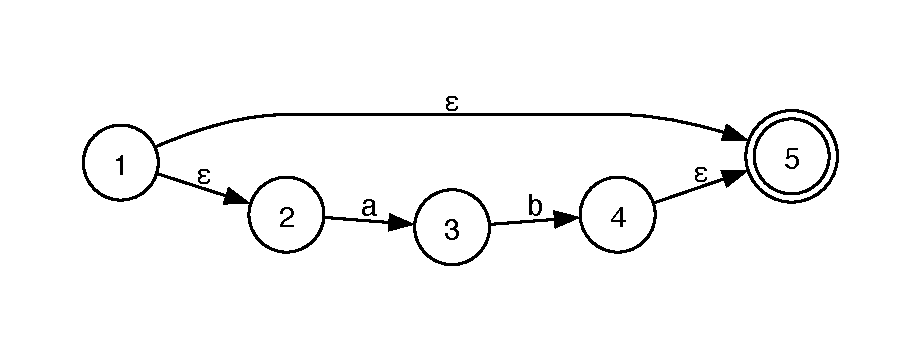
\includegraphics[width=\textwidth]{ab.pdf}
\end{figure}

$bc^*$
\begin{figure}[htp]
    \centering
    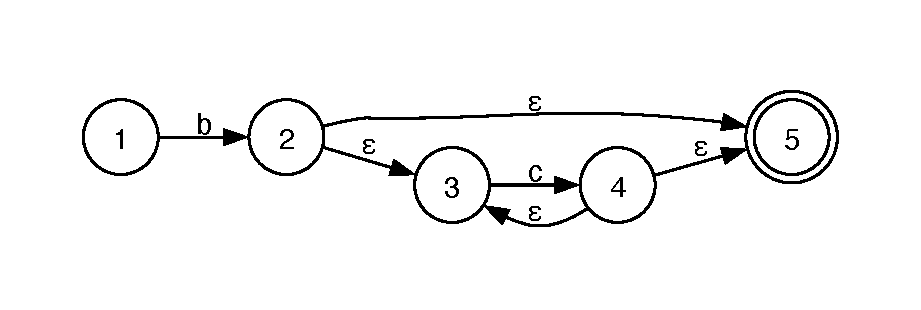
\includegraphics[width=\textwidth]{bc.pdf}
\end{figure}

% \digraph{bc}{
%     fontname="Helvetica,Arial,sans-serif"
% 	node [fontname="Helvetica,Arial,sans-serif"]
% 	edge [fontname="Helvetica,Arial,sans-serif"]
%     rankdir=LR;
%     size="8,5";
%     node [shape = doublecircle]; 5;
%     node [shape = circle];
%     1->2  [label = "b"];
%     1->5 [label = "ε"];
%     2->3 [label = "ε"];
%     3->4 [label = "c"];
%     4->3 [label = "ε"];
%     4->5 [label = "ε"];

% }

$ac$

% \digraph{ac}{
%     fontname="Helvetica,Arial,sans-serif"
% 	node [fontname="Helvetica,Arial,sans-serif"]
% 	edge [fontname="Helvetica,Arial,sans-serif"]
%     rankdir=LR;
%     size="8,5";
%     node [shape = doublecircle]; 3;
%     node [shape = circle];
%     1->2  [label = "a"];
%     2->3 [label = "b"];
% }
\begin{figure}[h]
    \centering
    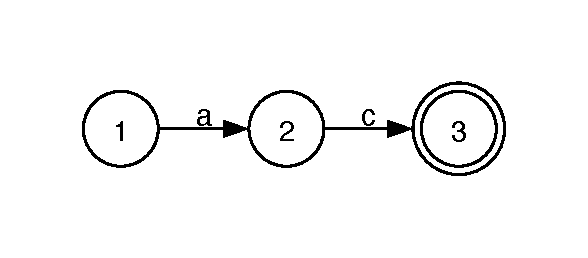
\includegraphics[width=\textwidth]{ac.pdf}
\end{figure}

\newpage
$\left(ab\right)?|bc^*|ac$

\begin{figure}[htp]
    \centering
    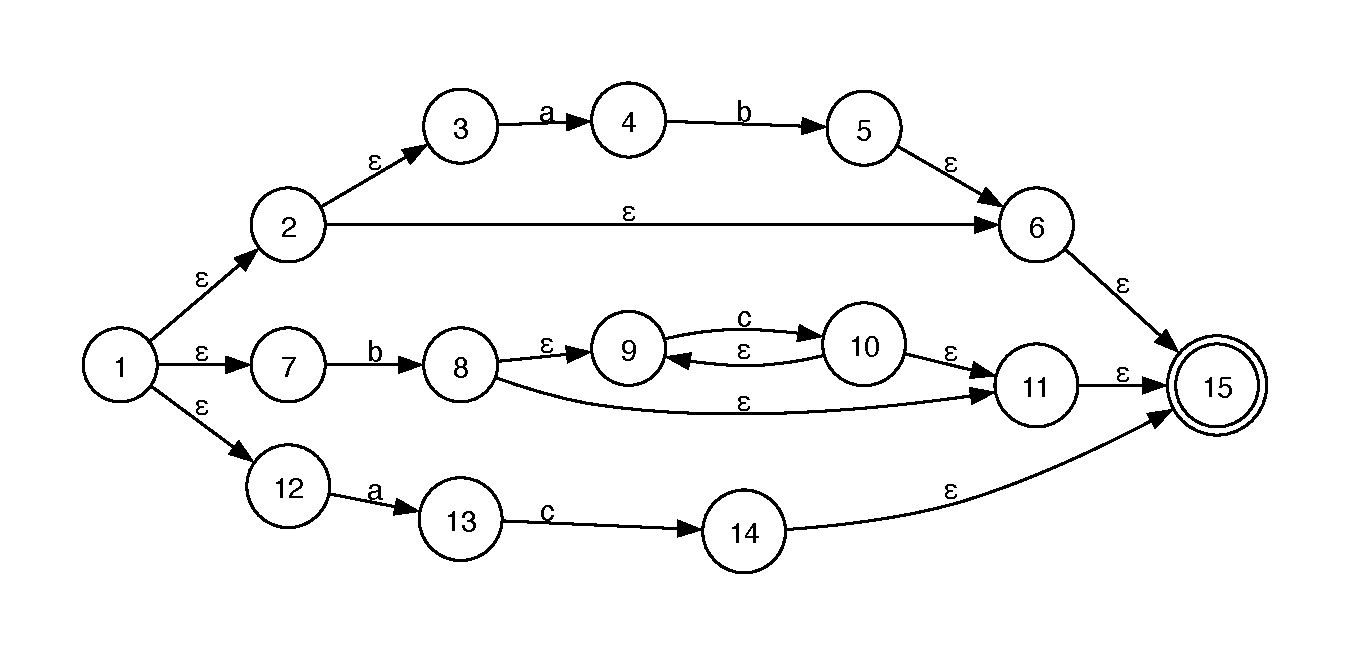
\includegraphics[width=\textwidth]{abc.pdf}
\end{figure}


% fontname="Helvetica,Arial,sans-serif"
% 	node [fontname="Helvetica,Arial,sans-serif"]
% 	edge [fontname="Helvetica,Arial,sans-serif"]
%     rankdir=LR;
%     size="8,5";
%     node [shape = doublecircle]; 15;
%     node [shape = circle];
%     1->2 [label = "ε"];
%     2->3 [label = "ε"];
%     2->6 [label = "ε"];
%     3->4 [label = "a"];
%     4->5 [label = "b"];
%     5->6 [label = "ε"];
%     1->7 [label = "ε"];
%     7->8 [label = "b"];
%     8->9 [label = "ε"];
%     10->9 [label = "ε"]
%     9->10  [label = "c"];
%     10->11 [label = "ε"];
%     8->11 [label = "ε"];
%     1->12 [label = "ε"];
%     12->13 [label = "a"];
%     13->14 [label = "c"];
%     14->15 [label = "ε"];
%     11->15 [label = "ε"];
%     6->15 [label = "ε"];

Уберем лишние $\varepsilon$\\

\begin{figure}[H]
    \centering
    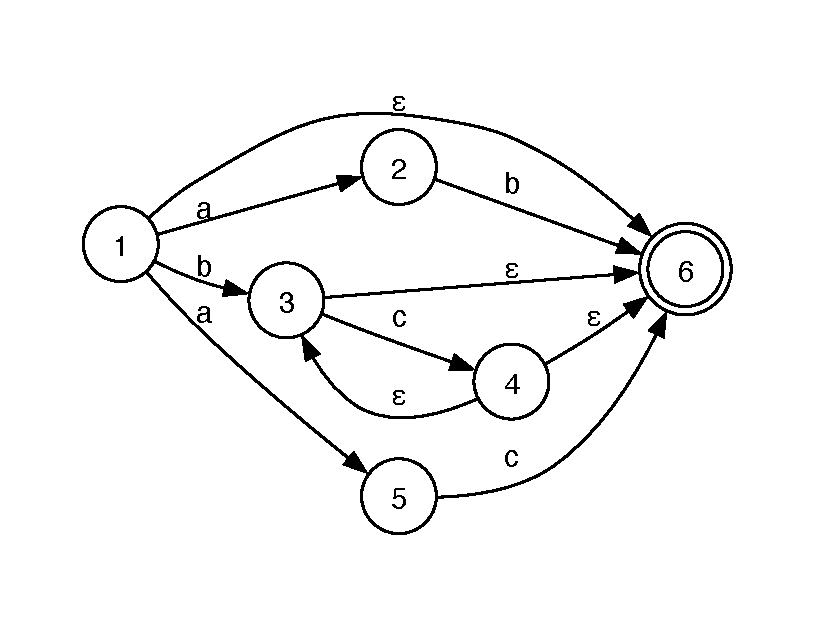
\includegraphics[width=\textwidth]{abcc.pdf}
\end{figure}

\section*{ДКА}

\begin{table}[H]
    \begin{tabular}{|l|l|l|l|l|}
    \hline
    N & State & a   & b   & c     \\ \hline
    1 & 1,6   & 2,5 & 3,6 & -     \\ \hline
    2 & 2,5   & -   & 6   & 6     \\ \hline
    3 & 3,6   & -   & -   & 3,4,6 \\ \hline
    4 & 6     & -   & -   & -     \\ \hline
    5 & 3,4,6 & -   & -   & 3,4,6 \\ \hline
    \end{tabular}
\end{table}
\includesvg{image/abc-d.svg}
\section*{Минимизация ДКА}
\begin{table}[H]
    \begin{tabular}{|llll|lll|lll|lll|}
    \hline
    \multicolumn{4}{|l|}{}                                                                  & \multicolumn{3}{l|}{$P_0$}                             & \multicolumn{3}{l|}{$P_1$}                             & \multicolumn{3}{l|}{$P_2$}                             \\ \hline
    \multicolumn{1}{|l|}{$\delta$} & \multicolumn{1}{l|}{a} & \multicolumn{1}{l|}{b} & c & \multicolumn{1}{l|}{a}  & \multicolumn{1}{l|}{b}  & c  & \multicolumn{1}{l|}{a}  & \multicolumn{1}{l|}{b}  & c  & \multicolumn{1}{l|}{a}  & \multicolumn{1}{l|}{b}  & c  \\ \hline
    \multicolumn{1}{|l|}{1}           & \multicolumn{1}{l|}{2} & \multicolumn{1}{l|}{3} & - & \multicolumn{1}{l|}{$B_0$} & \multicolumn{1}{l|}{$A_0$} & -  & \multicolumn{1}{l|}{$C_1$} & \multicolumn{1}{l|}{$B_1$} & -  & \multicolumn{1}{l|}{$C_2$} & \multicolumn{1}{l|}{$B_2$} & -  \\ \hline
    \multicolumn{1}{|l|}{2}           & \multicolumn{1}{l|}{-} & \multicolumn{1}{l|}{4} & 4 & \multicolumn{1}{l|}{-}  & \multicolumn{1}{l|}{$A_0$} & $A_0$ & \multicolumn{1}{l|}{-}  & \multicolumn{1}{l|}{$D_1$} & $D_1$ & \multicolumn{1}{l|}{-}  & \multicolumn{1}{l|}{$D_2$} & $D_2$ \\ \hline
    \multicolumn{1}{|l|}{3}           & \multicolumn{1}{l|}{-} & \multicolumn{1}{l|}{-} & 5 & \multicolumn{1}{l|}{-}  & \multicolumn{1}{l|}{-}  & $A_0$ & \multicolumn{1}{l|}{-}  & \multicolumn{1}{l|}{-}  & $B_1$ & \multicolumn{1}{l|}{-}  & \multicolumn{1}{l|}{-}  & $B_2$ \\ \hline
    \multicolumn{1}{|l|}{4}           & \multicolumn{1}{l|}{-} & \multicolumn{1}{l|}{-} & - & \multicolumn{1}{l|}{-}  & \multicolumn{1}{l|}{-}  & -  & \multicolumn{1}{l|}{-}  & \multicolumn{1}{l|}{-}  & -  & \multicolumn{1}{l|}{-}  & \multicolumn{1}{l|}{-}  & -  \\ \hline
    \multicolumn{1}{|l|}{5}           & \multicolumn{1}{l|}{-} & \multicolumn{1}{l|}{-} & 5 & \multicolumn{1}{l|}{-}  & \multicolumn{1}{l|}{-}  & $A_0$ & \multicolumn{1}{l|}{-}  & \multicolumn{1}{l|}{-}  & $B_1$ & \multicolumn{1}{l|}{-}  & \multicolumn{1}{l|}{-}  & $B_2$ \\ \hline
    \end{tabular}
    \end{table}

$$P_0 = { A_0 = <1,3,4,5>, B_0 = <2>}$$
$$P_1 = { A_1 = <1>, B_1 = <3,5>, C_1 = <2>, D_1 = <4>}$$
$$P_2 = { A_2 = <1>, B_2 = <3,5>, C_2 = <2>, D_2 = <4>}$$


\begin{figure}[H]
    \centering
    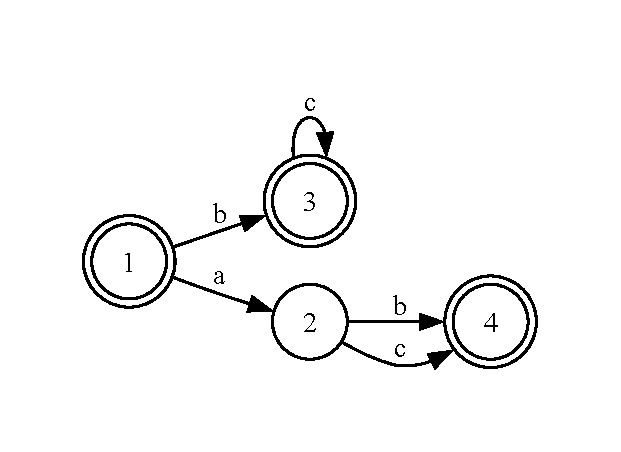
\includegraphics[width=0.7\textwidth]{abc-m.pdf}
\end{figure}
\section*{Программа-распознаватель}
\subsection*{Код}
\lstinputlisting[style=listing]{main.py}
\subsection*{Вывод}
\begin{verbatim}
True
True
True
True
True
False
False
False
\end{verbatim}



\end{document}